Any blade of a wind turbine is composed from root to tip of a smooth distribution of cross sections, much like the one illustrated in figure \labelcref{subfig:zukovsky_foil}.
Referred to as airfoils, these cross sections are optimized for the generation of lift.
As was alluded to in the section on complex analysis, these are wholly two dimensional objects, whose ability to generate lift can be quantified by the means of this theory.
Their mathematical representation warrants discussion, as it lends itself to the impending numerical analysis by way of comparison to theoretically derived values.
Consider then the complex variable $\ezh^{\prime} = x^{\prime} + i z^{\prime}$ whose values trace the circle centered at the origin of radius $c$.
The \textsc{Žukvoskij} transform takes a complex value and maps it to the point%
\footnote{%
  \cite{schlichting1967aerodynamiki} \textsc{Schlichting} \& \textsc{Truckenbrodt}, p.404, eq.6.37
}
\begin{equation}\label{eq:zukovsky_map}
  \ezh = f(\ezh^{\prime}) = \ezh^{\prime} + \frac{c^2}{\ezh^{\prime}}.
\end{equation}

\noindent
Expressing the variables in terms of their polar representations $x^{\prime} = r \cos{\theta}$ and $z^{\prime} = r \sin{\theta}$ yields
\begin{subequations}\label{eq:zukovsky_ellipse}
        \begin{equation}\tag{\theequation{a, b}}
          x = \left( r + \frac{c^2}{r} \right) \cos{\theta}, \qquad z = \left( r - \frac{c^2}{r} \right) \sin{\theta}.
        \end{equation}
\end{subequations}

\noindent
This constitutes an ellipse, as upon squaring the equations \subeqref{\ref{eq:zukovsky_ellipse}}[a, b], and adding them, we find that
\begin{subequations}\label{eq:ellipse_equations}
        \begin{equation}\tag{\theequation{a, b, c}}
          \frac{x^2}{a^2} + \frac{z^2}{b^2} = 1, \qquad a = r + \frac{c^2}{r}, \qquad b = \left\vert r - \frac{c^2}{r} \right\vert.
        \end{equation}
\end{subequations}

The airfoils of \textsc{von Kármán} \& \textsc{Trefftz} are generalizations of those of \textsc{Žukovskij}.%
\footnote{%
        \cite{prandtl1957applied} \textsc{Prandtl} \& \textsc{Tietjens}, \S106, pp.182--185
}

\begin{equation}
  \frac{\ezh - 2c}{\ezh + 2c} = \frac{{(\ezh^{\prime} - c)}^2}{{(\ezh^{\prime} + c)}^2}
\end{equation}

\noindent
It can be shown%
\footnote{%
        \cite{milne-thomson1958aerodynamics} \textsc{Milne-Thomson}, pp.125--128
}
that this is equivalent to the expression

\begin{equation}
  \frac{\ezh}{kc} = \frac{{(\ezh^{\prime} + c)}^k + {(\ezh^{\prime} - c)}^k}{{(\ezh^{\prime} + c)}^k - {(\ezh^{\prime} - c)}^k}.
\end{equation}

\begin{figure}[h]
  \centering
  \begin{subfigure}{.45\textwidth}
    \centering
    \scalebox{1}{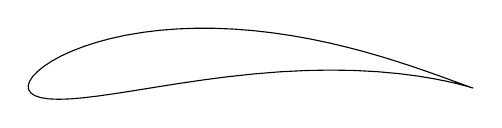
\begin{tikzpicture}
	\begin{scope}[scale = 1]
		\draw (2.758788561716295, 0.014308681190452949)
		     --(2.695225892989764, 0.037092154898239194)
		     --(2.605349631772322, 0.06979565712747693)
		     --(2.4914837918368695, 0.11134581613267103)
		     --(2.355902921626414, 0.1603737295619958)
		     --(2.2008045814183324, 0.21530771855934483)
		     --(2.028299068447968, 0.27445634630396487)
		     --(1.8404107881627163, 0.3360797670868505)
		     --(1.6390866090592162, 0.3984491156551494)
		     --(1.4262076116060918, 0.4598946527632113)
		     --(1.2036016566330967, 0.5188439025661553)
		     --(0.9730550610036036, 0.5738512022129862)
		     --(0.73632234899597, 0.623620060559015)
		     --(0.495133554475756, 0.6670195858704349)
		     --(0.2511989071110874, 0.7030960560405968)
		     --(0.0062109763365571675, 0.7310805091921784)
		     --(-0.23815550112870126, 0.7503930499721028)
		     --(-0.48024579571179227, 0.7606444078864456)
		     --(-0.7184290019027861, 0.7616351518248976)
		     --(-0.9511031222448073, 0.753352858418116)
		     --(-1.1767010455574276, 0.7359674478355478)
		     --(-1.3936970605036954, 0.7098248349723357)
		     --(-1.6006135663549095, 0.6754389924569452)
		     --(-1.7960276676795595, 0.6334824805412028)
		     --(-1.978577367463463, 0.5847754641282181)
		     --(-2.1469671037607583, 0.5302732058422353)
		     --(-2.299972409220211, 0.4710519935351507)
		     --(-2.4364435124278963, 0.4082934288729404)
		     --(-2.5553077475237425, 0.3432669691792857)
		     --(-2.6555706974927373, 0.2773105768485559)
		     --(-2.7363160714457173, 0.2118092897902284)
		     --(-2.7967044127444707, 0.1481714845436572)
		     --(-2.835970859726851, 0.08780256525696889)
		     --(-2.8534223415964473, 0.032075784385500086)
		     --(-2.848434796404079, -0.017700102798287633)
		     --(-2.8204512522478913, -0.06031660912926762)
		     --(-2.7689819191450327, -0.09470486309736903)
		     --(-2.693607791463116, -0.11997847030261366)
		     --(-2.5939896385026984, -0.13547946032443703)
		     --(-2.4698846191332704, -0.140826320023287)
		     --(-2.3211730158031574, -0.1359622874148969)
		     --(-2.1478976183674963, -0.12120096278896286)
		     --(-1.9503179212971546, -0.09726489676819827)
		     --(-1.728980305675844, -0.06531123562771457)
		     --(-1.4848035236783015, -0.026936975462191093)
		     --(-1.2191759113780511, 0.01584468714471865)
		     --(-0.9340568306150272, 0.060665412677036956)
		     --(-0.6320702284625005, 0.10490687697536827)
		     --(-0.31657374074855554, 0.14585243739251808)
		     --(0.008316175538151206, 0.18088068385602307)
		     --(0.33776230721800793, 0.20768701506209997)
		     --(0.6663221249329712, 0.22450959781216961)
		     --(0.9881444104189271, 0.23032846733124046)
		     --(1.2972363810801255, 0.225004244229849)
		     --(1.587775150982404, 0.20932830116194534)
		     --(1.854425397604547, 0.18496938523517836)
		     --(2.0926208069160066, 0.15432004316127923)
		     --(2.298772263168712, 0.12026482044310205)
		     --(2.4703796026735434, 0.0859057865526468)
		     --(2.6060419620315205, 0.0542858573109235)
		     --(2.705379061834188, 0.02814609469700352)
		     --(2.7688878599434776, 0.009742075599795008)
		     --(2.797763911112366, 0.0007305548454568239)
		     --(2.7937150187611346, 0.0021249002378133514)
		     --cycle;
	\end{scope}
\end{tikzpicture}}
    \caption{\textsc{Žukovskij} airfoil}
    \label{subfig:zukovsky_foil}
  \end{subfigure}
  \begin{subfigure}{.45\textwidth}
    \centering
    \scalebox{1}{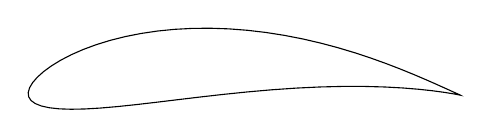
\begin{tikzpicture}
	\begin{scope}[scale = 1]
		\draw (2.67129737943394, 0.01981414579319518)
		--(2.6055930177904445, 0.04950831501891657)
		--(2.514783709175962, 0.09067900363003957)
		--(2.4015239958010404, 0.14155793453136303)
		--(2.268173782818535, 0.20020997876115854)
		--(2.1168710337951344, 0.2646126673933586)
		--(1.949581422653599, 0.3327277145824164)
		--(1.7681389745048341, 0.4025593492381791)
		--(1.5742806055961682, 0.47219977503625493)
		--(1.3696750012251067, 0.5398635822881194)
		--(1.1559458891717507, 0.6039132014025863)
		--(0.9346898911325553, 0.6628773102595525)
		--(0.707489325820905, 0.7154637854345509)
		--(0.47592047941396265, 0.76056844641333)
		--(0.24155793607236475, 0.7972805355643885)
		--(0.005975586010149726, 0.8248856227313639)
		--(-0.22925508146886023, 0.842866423317455)
		--(-0.4625688224718493, 0.8509018667620705)
		--(-0.6924120819595215, 0.8488646398383144)
		--(-0.9172495382058669, 0.8368173474056237)
		--(-1.1355712883313767, 0.8150073739998162)
		--(-1.3459002476351156, 0.7838604857588082)
		--(-1.5467993612640805, 0.7439731773293213)
		--(-1.7368782446202147, 0.6961037366929703)
		--(-1.9147988776064726, 0.6411619662046033)
		--(-2.0792799754066493, 0.5801974531500982)
		--(-2.22909964146573, 0.5143862169497124)
		--(-2.363095870460264, 0.4450154538723774)
		--(-2.4801644003022316, 0.37346591618356634)
		--(-2.5792533010721383, 0.30119111804987736)
		--(-2.659353545723536, 0.22969185759454236)
		--(-2.7194848001418945, 0.1604829929557973)
		--(-2.7586768112750804, 0.09504587100865389)
		--(-2.7759539543845544, 0.03475297130804453)
		--(-2.7703587812458896, -0.019248436851715886)
		--(-2.7410841011865665, -0.06613819173957096)
		--(-2.6876457790906274, -0.10535773659257959)
		--(-2.6098777138758793, -0.13645528150978586)
		--(-2.5078235299139564, -0.1590590326725153)
		--(-2.3816818776405717, -0.1729366889662201)
		--(-2.231804693515952, -0.17805724654415528)
		--(-2.0587193319087884, -0.174637260302784)
		--(-1.8631625759982529, -0.16317248702274756)
		--(-1.6461227611519977, -0.1444555140412429)
		--(-1.4088880866428837, -0.11957790072505473)
		--(-1.153098690268948, -0.08991410586293296)
		--(-0.8807986422469001, -0.057084149878539825)
		--(-0.5944822288530751, -0.02289257676407962)
		--(-0.29712714489111836, 0.01075708480956793)
		--(0.007794033159036052, 0.04197047944084678)
		--(0.316332910788329, 0.06898774732474992)
		--(0.6241222854759326, 0.09031654500634659)
		--(0.9264751653676351, 0.1048596294055946)
		--(1.2185246432014436, 0.11202155650687179)
		--(1.4953970292987568, 0.1117790883741735)
		--(1.752404176636463, 0.10470293117531068)
		--(1.9852359298122229, 0.09192436789579289)
		--(2.190131407046079, 0.07504827684792356)
		--(2.3640089029517104, 0.056022348441002554)
		--(2.504537694666027, 0.03697930599737796)
		--(2.610137542670863, 0.02007361793172077)
		--(2.6798817337160634, 0.0073381627276980456)
		--(2.7131836496021915, 0.0006063883540200069)
		--(2.708778327465989, 0.003141197677375565)
		--cycle;
	\end{scope}
\end{tikzpicture}}
    \caption{\textsc{von Kármán}--\textsc{Trefftz} airfoil}
    \label{subfig:karman-trefftz_foil}
  \end{subfigure}
  \caption{%
        (a) \textsc{Žukovsky} and (b) \textsc{von Kármán}--\textsc{Trefftz} airfoils, whose parameters are $c = 1.4$ and $s = \sfrac{1}{4}(i -\sfrac{3}{5})$.
        The $k = 1.94$
        }
  \label{fig:analytic_foils}
\end{figure}
